\section{Analysing Data}
\hbox{Scatter plots of all the input parameters are plotted with the output parameter(Strength).}
\begin{center}
    \begin{tabular}{cc}
        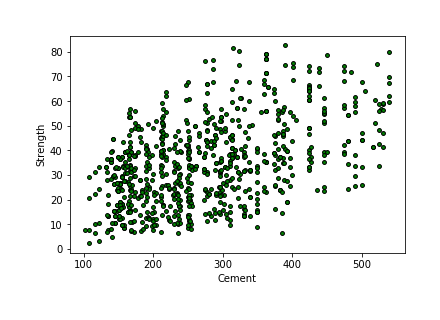
\includegraphics[scale=0.5]{images/Plot_01.png}&
        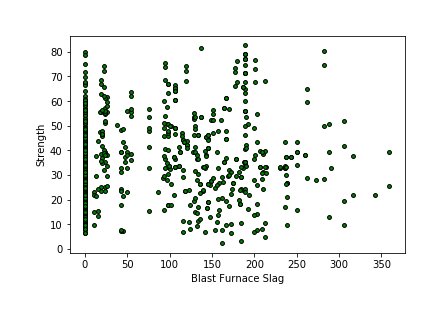
\includegraphics[scale=0.5]{images/Plot_02.png}\\
        a) & b)\\
        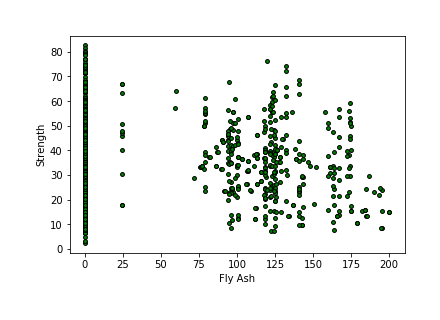
\includegraphics[scale=0.5]{images/Plot_03.png}&
        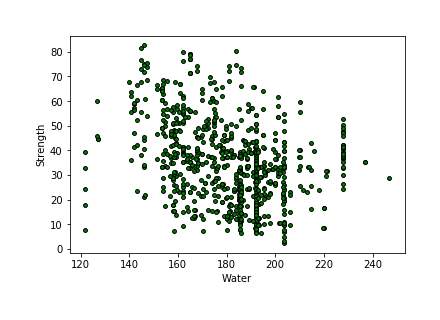
\includegraphics[scale=0.5]{images/Plot_04.png}\\
        c) & d)\\
    \end{tabular}
    \captionof{figure}{Scatter the plots between Strength and a) cement; b) Blast Furnace Slag; c) Fly Ash; d) Water;}
\end{center}
It can be noted that the data is real valued except for Age which is integer valued and it is hard to visualize any linear relationship between input parameters and strength. As it is already mentioned that the relation between strength and input parameters is highly non-linear the a graphs are as expected.\\
For the Cement it can be seen that with the increase of value of cement there is increase in strength but it can also be noted that the strength is highly affected by other parameters as even for high cement values, around $500kgm^{-3}$, strength value varies low to high, around $40MPa$ to $80MPa$.
\begin{center}
    \begin{tabular}{cc}
        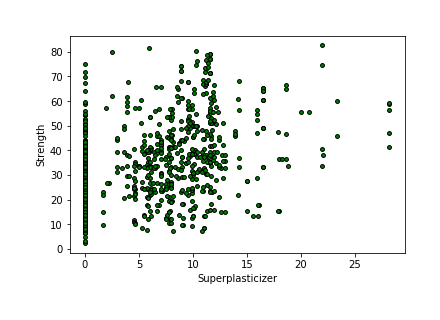
\includegraphics[scale=0.5]{images/Plot_05.png}&
        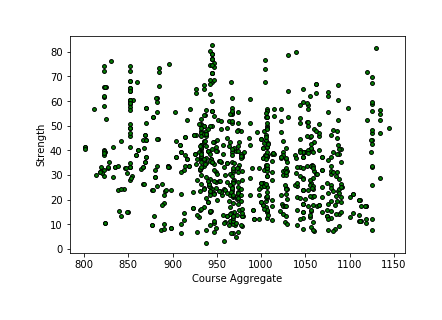
\includegraphics[scale=0.5]{images/Plot_06.png}\\
        a) & b)\\
        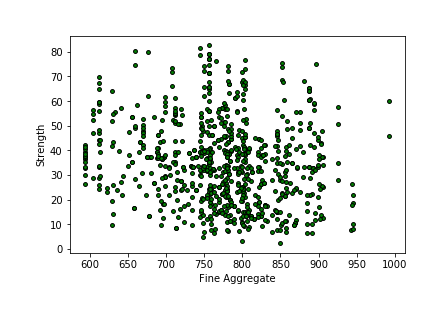
\includegraphics[scale=0.5]{images/Plot_07.png}&
        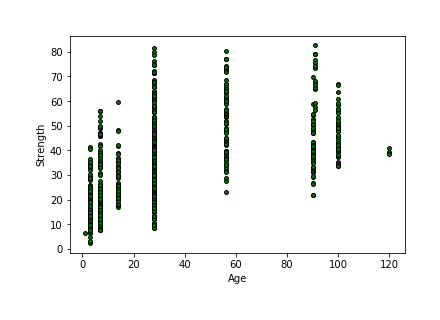
\includegraphics[scale=0.5]{images/Plot_08.png}\\
        c) & d)\\
    \end{tabular}
    \captionof{figure}{Scatter plots between strength and a) Superplasticizer; b) Coarse Aggregate; c) Fine Aggregate; d) Age}
\end{center}

Now the values of data are presented in table to see the maximum, minimum, mean and median of the data in their respective units as discussed in Table 1.1. This tells us the need of normalization of the data as values are not varying in same range and this can lead to baises in prediction. For example cement is ranging form 102 to 540 $kgm^{-3}$ and superplasticizer is ranging from 0 to 22.1 $kgm^{-3}$ this may lead to biases toward cement values.
\begin{center}
    \begin{tabular}{|c|c|c|c|c|}
    	\hline
        $attribute$ & $minimum$ & $maximum$ & $Average$ & $median$\\
        \hline
        $Cement$ & 102.0 & 540.0 & 277.093 & 257.75\\
        \hline
        $Blast Furnace Slag$ & 0.0 & 342.1 & 76.9958 & 22.0\\
        \hline
        $Fly Ash$ & 0.0 & 195.0 & 57.6307 & 0.0\\
        \hline
        $Water$ & 127.0 & 228.0 & 180.1824 & 183.0\\
        \hline
        $Superplasticizer$ & 0.0 & 22.1 & 6.4395 & 7.0\\
        \hline
        $Coarse Aggregate$ & 801.0 & 1145.0 & 976.1921 & 972.2\\
        \hline
        $Fine Aggregate$ & 594.0 & 945.0 & 774.1864 & 778.25\\
        \hline
        $Age$ & 1.0 & 120.0 & 32.3507 & 28.0\\
        \hline
        $Strength$ & 2.33 & 79.4 & 35.415 & 33.724\\
        \hline
    \end{tabular}
	\captionof{table}{Aspect of components of data}
\end{center}

\section{Model Architecture}
The Artificial Neural Network model with one input layer, one hidden layer, and one output layer was considered for the analysis. Model is fully connected network with batch mode of training. The number of input and ouput neurons is 8 and 1 respectively and decided by the number of input and ouput parameters. Number of hidden neurons can be varied.\\
\begin{figure}[h]
	\begin{center}
		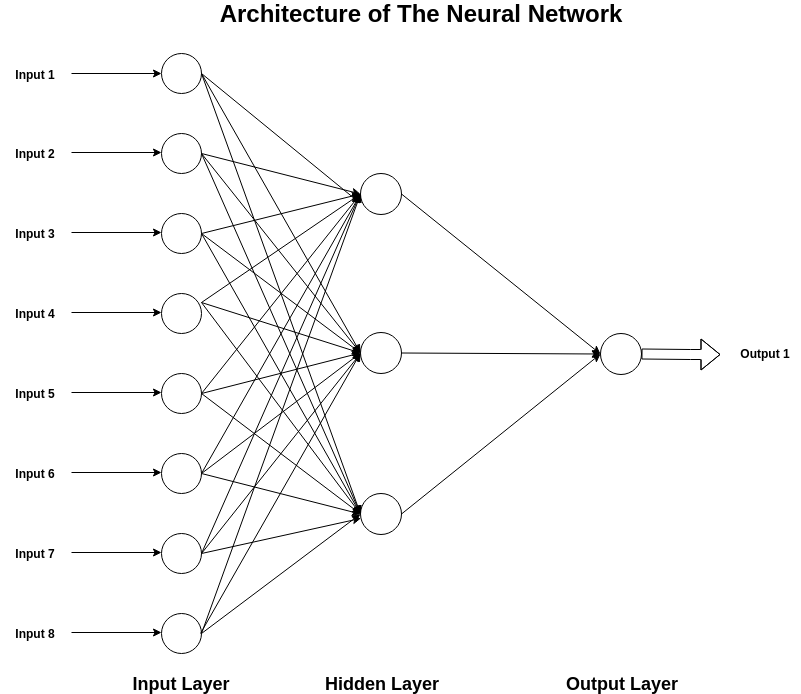
\includegraphics[scale=0.5]{images/architecture.png}
		\captionof{figure}{Architecture of neural network}
	\end{center}
\end{figure}
As the ouput parameter is Strength which is real valued transfer function for both hidden and ouput layer was selected as log sigmoid transfer funciton with a = 1. The values of input parameters were normalized within range -4 to 4 for all parameters before feeding into the network. Also the target values are normalized in the range 0.1 to 0.9.
\begin{center}
		{\huge $y = \frac{1}{1 + e^{-ax}}$}
		\captionof{figure}{Log sigmoid transfer function}
\end{center}


\section{Model Parameters}
Number of hidden neurons, learining rate, momentum coefficient and tolerance value are the model parameters which can be changed to alter the convergence rate and termination criterion of the training. These values were chosen by trial and error method.\\
Different sets of data was feed into the neural network with different model parameters and then number of interations were noted for a given torelance value. Model parameters which gave the best results i.e. minimum number of iterations were chosen as final parameters.\\
\begin{center}
	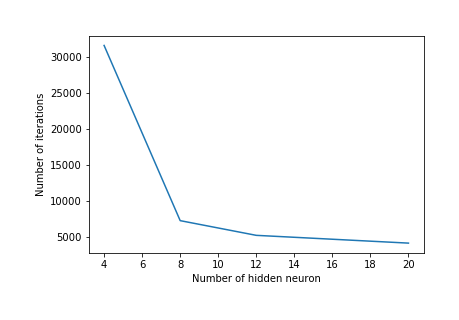
\includegraphics[scale=0.8]{images/iterations/Plot_01.png}
	\captionof{figure}{Comparison of number of iterations for tolerance = $10^{-5}$, learning rate = 0.3 and momentum coefficient = 0}
\end{center}
First the value of learning rate and momentum coefficients were fixed and for hidden neurons 4, 8, 12 and 20 the training was performed and the number of interation taken for training were noted.\\
\begin{center}
	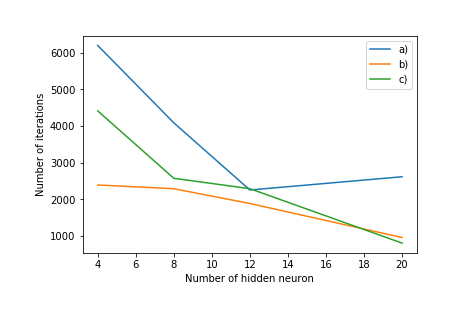
\includegraphics[scale=0.8]{images/iterations/Plot_02.png}
	\captionof{figure}{Comparison of number of iterations for tolerance = $10^{-5}$ and\\ a)learning rate = 0.3 and momentum coefficient = 0\\
		b)learning rate = 0.7 and momentum coefficient = 0.5\\
		c)learning rate = 0.9 and momentum coefficient = 0.6}
\end{center}
Then the values for learning rate and momentum was increased and for different number of hidden neurons again the number of iterations were noted. This process was repeated for various values of model parameters. For this procedure the value of tolerance was taken as $10^{-5}$ but after the selection of parameters the value of tolerance was further decreased to $5\times10^{-6}$ as this increased the accuracy in prediction and increase in number of iterations was not much. But further reduction in tolerance value increased the number of iteration very much.\\
\begin{center}
	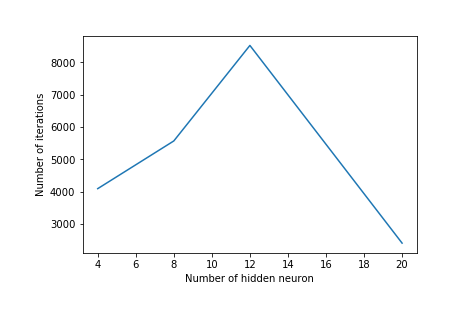
\includegraphics[scale=0.8]{images/iterations/Plot_03.png}
	\captionof{figure}{Comparison of number of iterations for tolerance = $5\times10^{-6}$, learning rate = 0.9 and momentum coefficient = 0.6}
\end{center}
For tolerance, it was noted that for tolerance value of $10^{-6}$ the results of training and testing were good and by further reduction in its value increased the number of iteration but there was not much improvement in predictions. For instance, with tolerance = $10^{-7}$ it took 10 to 20 times more iterations to converge than with tolerance value of $10^{-6}$, but the Mean Square Error for testing in both the cases was of order $10^{-6}$.
\begin{center}
	\begin{tabular}{|c|c|}
		\hline
		\textbf{Model Parameter} & \textbf{Value} \\
		\hline
		No. of Hidden Neurons & 20\\
		\hline
		Learining Rate & 0.9\\
		\hline
		Momentum Coefficients & 0.6\\
		\hline
		Error/Tolerance & $5\times10^{-6}$\\
		\hline
	\end{tabular}
	\captionof{table}{Decided Values of Parameters}
\end{center}